\documentclass{beamer}
\usepackage{tikz}
\usepackage{amsmath}
\usepackage{amssymb}
\usepackage{hyperref}
\usepackage{enumitem}
\usetikzlibrary{arrows}

\title{Mandelbrot Set Explorer}
\author{Jack DeSerrano}
\setlist[itemize]{leftmargin=*, label={}}
\date{\today}

\newcommand{\R}{\mathbb{R}}
\newcommand{\C}{\mathbb{C}}


\begin{document}

\frame{\titlepage}

\section[Outline]{}
\frame{\tableofcontents}

\section{Prerequisites}
\subsection{Complex numbers}
\frame
{
\begin{itemize}
\item <1-> Fundamental theorem of algebra (Gauss): An $n$-degree polynomial has $n$ roots.\\\text{}\\

\item <2->We can visualize the real numbers, $\R$, on a number line:

$$
\begin{tikzpicture}
\draw[<->] (-4, 0) -- (4, 0) node[right] 
{$\R$};
\foreach \n in  {
	-3.5,
	-1,
	0,
	1.4142135623730951, 
	3.141592653589793
	} 
\draw[shift = {(\n, 0)}, color = black] (0pt, 3pt) -- (0pt, -3pt);

\draw[shift = {(-3.5, 0)}, color = black] (0pt, 0pt) -- (0pt, -3pt) node [below] 
{$-7/5$};
\draw[shift = {(-1, 0)}, color = black] (0pt, 0pt) -- (0pt, -3pt) node [below] 
{$-1$};
\draw[shift = {(0, 0)}, color = black] (0pt, 0pt) -- (0pt, -3pt) node [below] 
{$0$};
\draw[shift = {(1.4142135623730951, 0)}, color = black] (0pt, 0pt) -- (0pt, -3pt) node [below] 
{$\sqrt 2$};
\draw[shift = {(3.141592653589793, 0)}, color = black] (0pt, 0pt) -- (0pt, -6pt) node [below] 
{$\pi$};

\end{tikzpicture}
$$

\item <3->Closure: $\R$ is closed under addition, subtraction, and multiplication, and $\R^\times$ is closed under division.\\\text{}\\

\item <4->What are the roots of $f(x) = x^2 +13$?\\\text{}\\

\item <5-> The fact that we can't determine any roots seems to contradict the fundamental theorem of algebra. Therefore, there must be something with which to equip the reals to make $f$ solvable. We call the ``equipped reals'' the \underline{complex numbers}, $\C$.
\end{itemize}
}


\frame
{
\begin{itemize}
\item<1-> In the complex numbers, we define $i = \sqrt{-1}$, called the \underline{imaginary unit}. \\\text{}\\ %This seemingly absurd axiom allows us to determine the roots of any polynomial! 

\item<2-> With this new tool, what are the roots of $f(z) = z^2 +13$? \\\text{}\\

\item<3-> The complex numbers are the algebraic closure of the reals. Extending the reals to the complex numbers is only natural, and it simply solves one of the two major problems with which the real numbers present us. \\\text{}\\ % Division by zero is the only problem that remains, though; there are well-defined solutions for zero division, but most times, we are okay without zero.

\item<4-> We can visualize $\R$ on a number line; analogously, we can visualize $\C$ on a two-dimensional plane, where the number line remains the same and the vertical axis is the number line times $i$.\\\text{}\\ 

\item<5-> Notation: $(a,\, b)$ is now $a +bi$ on the complex plane. If $z = a + bi$,  $a$ is the real part and $b$ is the imaginary part of $z$. For now, think of $z$ as a two-dimensional vector.
\end{itemize}
}

\frame
{

$$
\begin{tikzpicture}
\draw [<->] (-3.5, 0) -- (3.5, 0) node [right] {$\R$};
\draw [<->] (0, -3.5) -- (0, 3.5) node [above] {$\R i$};

\foreach \n in {-3,...,-1,1,2,...,3} {
\draw (\n,-3pt) -- (\n,3pt)   node [above] {$\n$};
}

\foreach \n in {-3,-2,2,3} {  
\draw (-3pt,\n) -- (3pt,\n)   node [right] {$\n i$};
}

\draw (-3pt, -1) -- (3pt, -1)   node [right] {$-i$};
\draw (-3pt, 1) -- (3pt, 1)   node [right] {$i$};

\draw[-latex] (0,0)--(3,2) node[right, black]{$z=\phantom{ 3 + 2i}$};

\end{tikzpicture}
$$

}

\frame
{

$$
\begin{tikzpicture}
\draw [<->] (-3.5,0) -- (3.5,0) node [right] {$\R$};
\draw [<->] (0,-3.5) -- (0,3.5) node [above] {$\R i$};

\foreach \n in {-3,...,-1,1,2,...,3} {
\draw (\n,-3pt) -- (\n,3pt)   node [above] {$\n$};
}

\foreach \n in {-3,-2,2,3} {  
\draw (-3pt,\n) -- (3pt,\n)   node [right] {$\n i$};
}

\draw (-3pt, -1) -- (3pt, -1)   node [right] {$-i$};
\draw (-3pt, 1) -- (3pt, 1)   node [right] {$i$};

\draw[-latex] (0,0)--(3,2) node[right, black]{$z = 3 + 2i$};

\end{tikzpicture}
$$

}

\frame
{
\begin{itemize}
\item <1->Magnitude of $z = a + bi$:
$$
|z| = \sqrt{a^2 + b^2}
$$
\item<2->Complex multiplication:
\begin{align*}
(a + bi)(c + di)	&= ac + adi + bci + bdi^2\\
		      	&= (ac - bd) + (ad + bc)i
\end{align*}
\item<3-> Complex conjugate of $z = a + bi$:
$$
\bar{z} = a - bi
$$
\item <4->Conjugate multiplication:
\begin{align*}
(a + bi)(a - bi)	&= a^2 - (bi)^2\\
			&= a^2 + b^2
\end{align*}
\end{itemize}
}

\subsection{Mandelbrot set}
\frame{
\begin{itemize}
\item <1-> Suppose $f(z) = z^2 + c$ where $c \in \C$. \\\text{}\\ 

\item <2->For each $c$, let us start with $f(0)$.\\\text{}\\ 

\item <3-> We take $f$ of this result, then take $f$ of that result, repeating the process {ad infinitum}.\\\text{}\\ 

\item <4-> When repeating this process, do the results shoot off to infinity (diverge) or stay bounded (converge or oscillate)?\\\text{}\\ 

\item <5-> This question determines whether a complex number $c$ is in the Mandelbrot set, i.e. if this repeated composition stays bounded, the number is in the set; otherwise, it is not. For complex numbers, we must look at the magnitudes of the results.\\\text{}\\

\item <6-> You just lost the game.
\end{itemize}
}

\frame
{
\begin{itemize}
\item <1->Example 1: is $c=1$ in the Mandelbrot set?
\item <2-> $$
f(0) = 0^2 + 1 = 1
$$ \vspace*{-32pt}
\item <3-> $$
f(1) = 1^2 + 1 = 2
$$ \vspace*{-32pt}
\item <4-> $$
f(2) = 2^2 + 1 = 5
$$ \vspace*{-32pt}
\item <5-> $$\ \,
f(5) = 5^2 + 1 = 26 
$$
\item <6-> Since the resulting numbers are growing without bound, $c=1$ is not in the Mandelbrot set.
\end{itemize}
}

\frame
{
\begin{itemize}
\item <1->Example 2: is $c=-1$ in the Mandelbrot set?
\item <2-> $$
f(0) = 0^2 - 1 = -1
$$ \vspace*{-32pt}
\item <3-> $$
f(-1) = (-1)^2 - 1 = 0 
$$ \vspace*{-32pt}
\item <4-> $$
f(0) = 0^2 - 1 = -1
$$ \vspace*{-32pt}
\item <5-> $$
f(-1) = (-1)^2 - 1 = 0 
$$
\item <6-> Since the resulting numbers are oscillating between $0$ and $-1$, $c=-1$ is in the Mandelbrot set. We say that $-1$ creates a cycle of period $2$.
\end{itemize}
}

\frame 
{
\begin{itemize}
\item <1->Example 3: is $c=i$ in the Mandelbrot set?
\item <2-> $$ \!\!\!\!\!\!\!\!\!
f(0) = 0^2 + i = i
$$ \vspace*{-32pt}
\item <3-> $$ \ \ \ 
f(i) = i^2 + i = -1+i 
$$ \vspace*{-32pt}
\item <4-> $$
f(-1 + i) = (-1 + i)^2 + i = -i
$$ \vspace*{-32pt}
\item <5-> $$\ \ \ \ \ 
f(-i) = (-i)^2 + i = -1 + i
$$ \vspace*{-32pt}
\item <6-> $$
f(-1 + i) = (-1 + i)^2 + i = -i
$$
\item <6-> Since the resulting numbers are oscillating between $-i$ and $-1 + i$, $c=i$ is in the Mandelbrot set. $i$ also creates a cycle of period $2$.
\end{itemize}
}

\frame
{
\begin{itemize}
\item <1->Example 4: is $c=2i$ in the Mandelbrot set?
\item <2-> $$\mkern-36mu \mkern-18mu \!\!
f(0) = 0^2 + 2i = 2i
$$ \vspace*{-32pt}
\item <3-> $$
f(2i) = (2i)^2 + 2i = -4 + 2i
$$ \vspace*{-32pt}
\item <4-> $$\,
f(-4 + 2i) = (-4 + 2i)^2 + 2i = 12 - 14i
$$ \vspace*{-32pt}
\item <5-> $$\ \ \ 
f(12 - 14i) = (12 - 14i)^2 - 1 = -52 - 334i 
$$
\item <6-> Since the magnitudes of the resulting numbers are growing without bound, $c=2i$ is not in the Mandelbrot set.
\end{itemize}
}

\frame
{
\begin{itemize}
\item <1->Now, let's go through every complex number, painting it black if it's in the Mandelbrot set, and white if it's not.\\\text{}\\

\item <2->Here is the result: % \url{https://commons.wikimedia.org/wiki/File:Mandelset_hires.png}

\item <3-> \begin{figure}
\centering
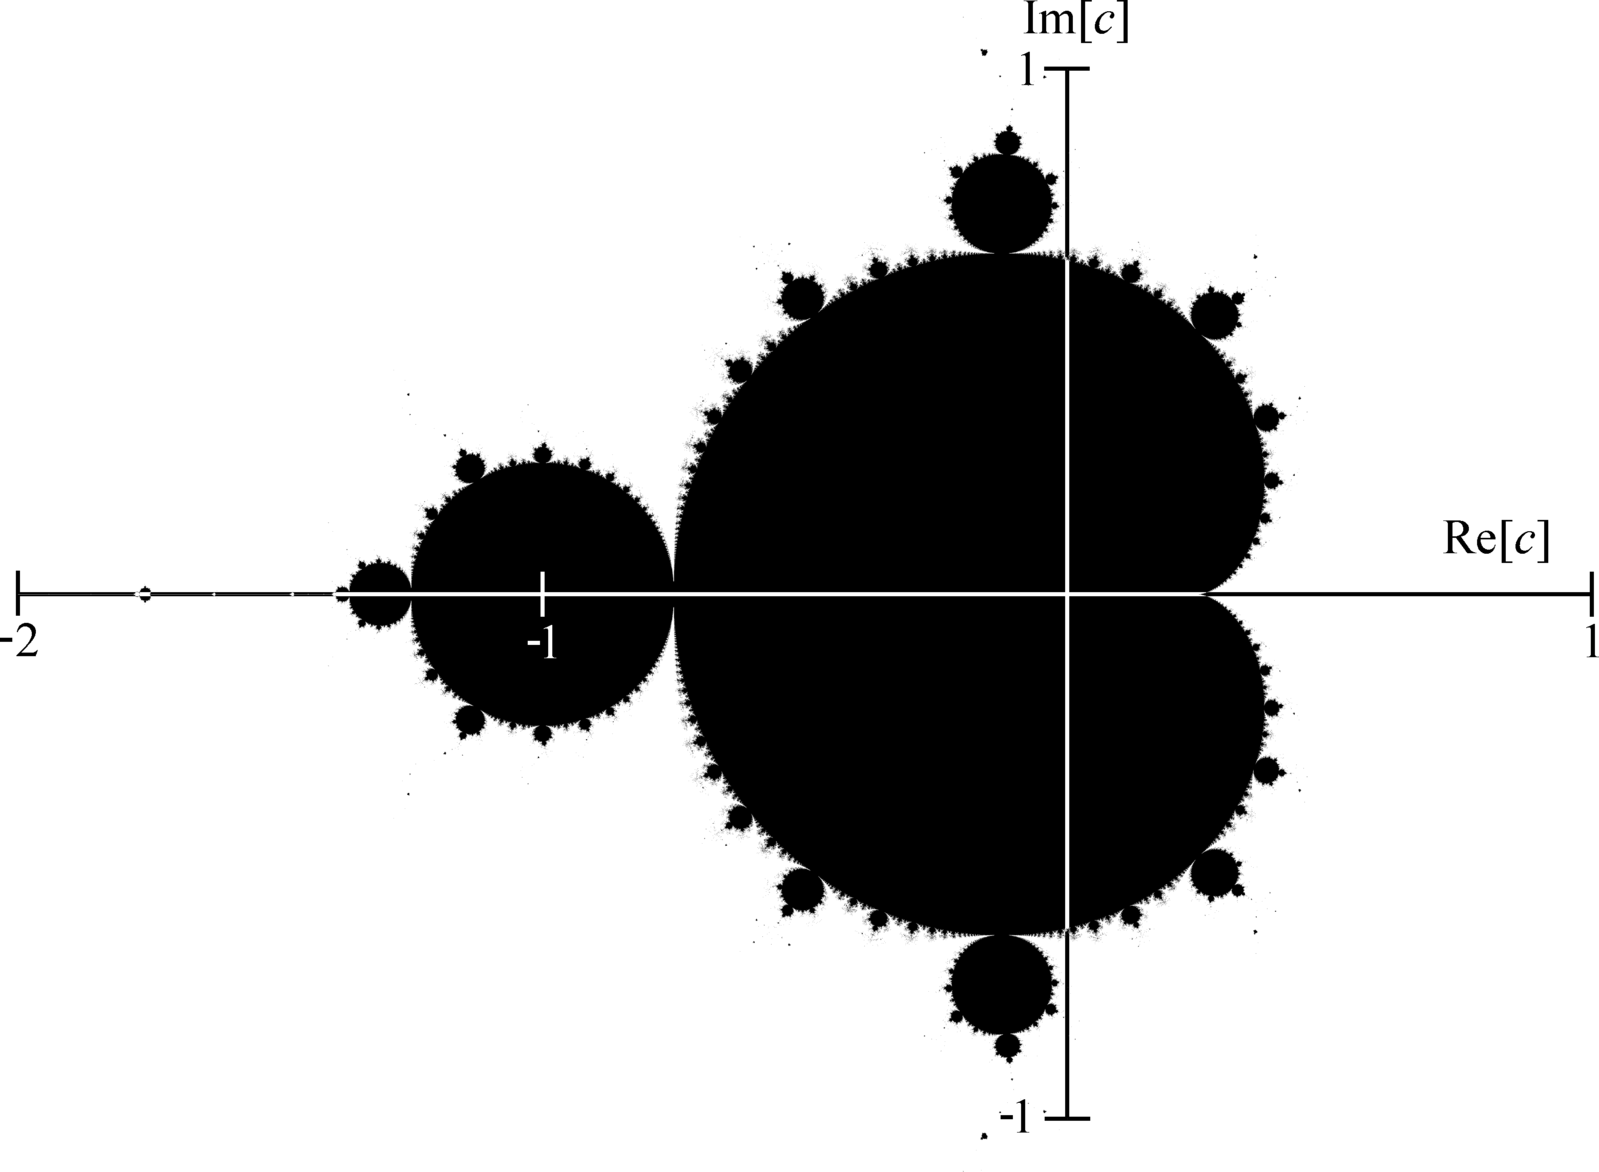
\includegraphics[scale=0.15]{presentation_images/mandelbrot_with_axis.png}
\end{figure}

\end{itemize}
}


\frame
{
\begin{itemize}
\item <1->It turns out that the Mandelbrot set looks even better when we colour points not in the set. We colour them based on how ``fast'' they go to infinity:
\item <2-> \begin{figure}
\centering
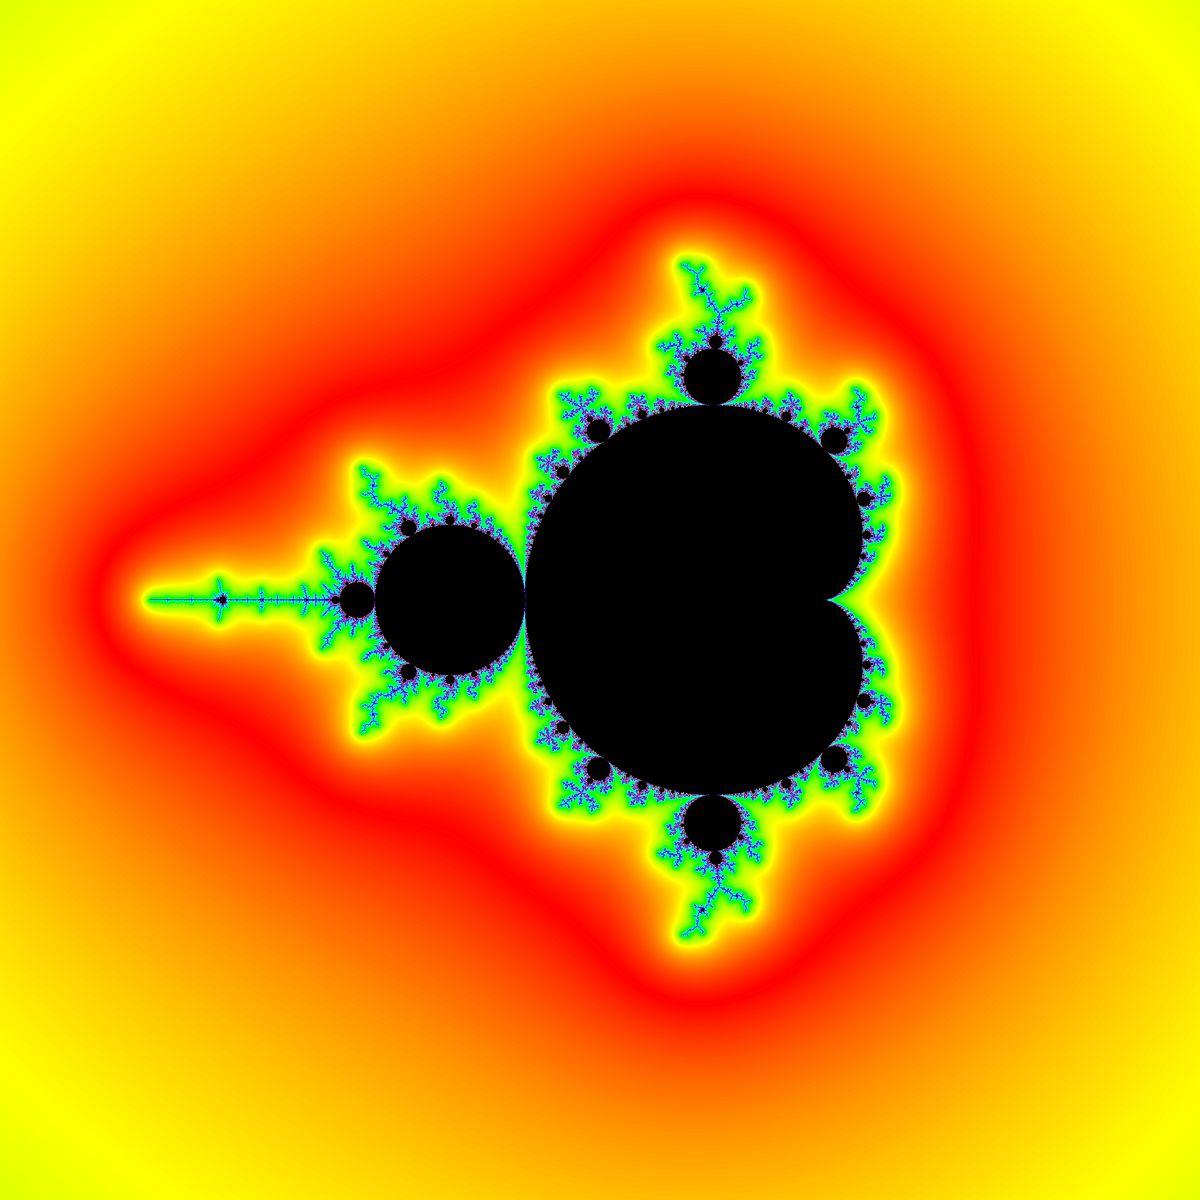
\includegraphics[scale=0.15]{presentation_images/mandelbrot_coloured.jpg} % \url{https://commons.wikimedia.org/wiki/File:Demm_2000_Mandelbrot_set.jpg}
\end{figure}
\end{itemize}
}

\section{}
\frame
{
\begin{itemize}
\item <1-> What I hoped to achieve with my program:\\\text{}\\
\item <2-> A program that allows the user to explore the Mandelbrot set, switch between a myriad of colourings, save zooms, reopen zooms, and generate Julia sets.
\end{itemize}
}

\frame
{
\begin{itemize}
\item <1-> What I learned:\\\text{}\\
\item <2-> Tkinter, NumPy array manipulation\\
\item <3-> Display methods\\
\item <4-> Various colouring methods/algorithms and the mathematics behind them\\
\item <5-> Patience\\
\item <6-> Ultimately, more mathematics than programming
\end{itemize}
}

\frame
{
\begin{itemize}
\item <1-> What I achieved:\\\text{}\\
\item <2-> A program that allows the user to explore the Mandelbrot set, switch between four colourings, save zooms, and reopen zooms.
\end{itemize}
}

\frame
{
\begin{itemize}
\item <1-> If I could've done it differently:\\\text{}\\
\item <2-> One colouring, but on a website\\
\item <3-> A completely different program
\end{itemize}
}

\frame
{
\begin{itemize}
\item <1-> If I had more time:\\\text{}\\
\item <2-> Learn more colouring algorithms\\
\item <3-> Make Julia sets\\
\item <4-> Implement on the web
\end{itemize}
}

\frame
{
Question period
}

\end{document}
